
%%%%%%%%%%%%%%%%%%%%%%% file typeinst.tex %%%%%%%%%%%%%%%%%%%%%%%%%
%
% This is the LaTeX source for then instructions to authors using
% the LaTeX document class 'llncs.cls' for contributions to
% the Lecture Notes in Computer Sciences series.
% http://www.springer.com/lncs       Springer Heidelberg 2006/05/04
%
% It may be used as a template for your own input - copy it
% to a new file with a new name and use it as the basis
% for your article.
%
% NB: the document class 'llncs' has its own and detailed documentation, see
% ftp://ftp.springer.de/data/pubftp/pub/tex/latex/llncs/latex2e/llncsdoc.pdf
%
%%%%%%%%%%%%%%%%%%%%%%%%%%%%%%%%%%%%%%%%%%%%%%%%%%%%%%%%%%%%%%%%%%%


\documentclass[runningheads,a4paper]{llncs}

\usepackage{amssymb}
\setcounter{tocdepth}{3}
\usepackage{float}
\usepackage{caption}
\usepackage{graphicx}
\graphicspath{{images/}}

\usepackage[]{booktabs}
\usepackage{hyperref}
\hypersetup{
    colorlinks=true,
    linkcolor=blue,
    filecolor=magenta,      
    urlcolor=blue,
}

\usepackage{url}
\urldef{\mailsa}\path|{alfred.hofmann, ursula.barth, ingrid.haas, frank.holzwarth,|
\urldef{\mailsb}\path|anna.kramer, leonie.kunz, christine.reiss, nicole.sator,|
\urldef{\mailsc}\path|erika.siebert-cole, peter.strasser, lncs}@springer.com|    
\newcommand{\keywords}[1]{\par\addvspace\baselineskip
\noindent\keywordname\enspace\ignorespaces#1}

\makeatletter
\newcommand{\printfnsymbol}[1]{%
  \textsuperscript{\@fnsymbol{#1}}%
}
\makeatother

\begin{document}

\mainmatter  % start of an individual contribution

% first the title is needed
\title{Recognizing Handshapes using Small and Unlabeled Datasets}

% a short form should be given in case it is too long for the running head
\titlerunning{Recognizing Handshapes using Small and Unlabeled Datasets}

% the name(s) of the author(s) follow(s) next
%
% NB: Chinese authors should write their first names(s) in front of
% their surnames. This ensures that the names appear correctly in
% the running heads and the author index.
%
\author{Ulises Jeremias Cornejo Fandos \inst{1}\thanks{equal contribution}%
\and Gaston Gustavo Rios \inst{1, 3}\printfnsymbol{1} \and \\ Franco Ronchetti \inst{1} \and Facundo Quiroga \inst{1} \and Waldo Hasperué \inst{1,2} \and Laura Lanzarini  \inst{1}}
%
\authorrunning{Cornejo \and Rios \and Ronchetti \and Quiroga \and Hasperué al.}


\def\aa{\}}
\def\ab{\{}

% the affiliations are given next; don't give your e-mail address
% unless you accept that it will be published
\institute{
$^{1}$ Facultad de Informática, Universidad Nacional de La Plata \\
$^{2}$  Investigador Asociado - Comisión de Investigaciones Científicas (CIC) \\
$^{3}$  Becario de entrenamiento - Comisión de Investigaciones Científicas (CIC)
 \\ \email{\ab ucornejo,grios,fquiroga,fronchetti,whasperue\aa @lidi.info.unlp.edu.ar}
}

%holooo
% NB: a more complex sample for affiliations and the mapping to the
% corresponding authors can be found in the file "llncs.dem"
% (search for the string "\mainmatter" where a contribution starts).
% "llncs.dem" accompanies the document class "llncs.cls".
%

\maketitle


\begin{abstract}
Advances in convolutional neural networks have  made possible significant  improvements in the state-of-the-art in image classification. However, their success on a particular field rests on the possibility of obtaining labeled data to train networks.  Handshape recognition from images,  an important subtask  of both gesture and sign language recognition,  suffers from such a lack of data.  Furthermore,  hands are highly deformable objects and therefore handshape classification  models require larger datasets.

We analyze both state-of-the-art models for image classification, as well as data augmentation schemes and specific models to tackle  problems with small datasets.  In particular,  we perform experiments with Wide-DenseNet, a state-of-the-art convolutional architecture and Prototypical Networks, a state-of-the-art few-shot learning meta model. In both cases, we also quantify the impact of data augmentation on accuracy. 

Our results show that on small and simple data sets such as CIARP,  all models and variations of achieve perfect accuracy,  and therefore the utility of the data is highly doubtful, despite its having 6000  samples. On the other hand, in small but complex datasets such as LSA16 (800 samples),  specialized methods such as Prototypical Networks do have an advantage over other methods.  On RWTH, another complex and small dataset with close to 4000 samples,  a  traditional and state-of-the-art method such as Wide-DenseNet surpasses  all other models.  Also, data augmentation consistently increases accuracy for Wide-DenseNet,  but not full  Prototypical Networks.

\keywords{ sign language, hand shape recognition,convolutional neural networks,densenet,  prototypical networks, small datasets}
\end{abstract}

        

\section{Introduction}


Hand shape recognition is a crucial component of any sign language recognition system. In recent years, new advances in machine learning   using models such as  convolutional neural networks  and recurrent neural s have improved our ability to tackle complex Recognition problems such as speech recognition. However, sign language recognition has not  been able to take advantage of most of these advances, since  the availability of labeled, quality data for training models is currently very limited \cite{}.   

In this article we propose to  employ and compare new methods devoted to deal with small and unlabeled data sets in order to improve the current state-of-the-art in hand shape recognition for sign language. 

our approach consists of combining and comparing three different techniques For improving model performance in these conditions: data augmentation,  prototipical learning and semi supervised learning.
for data augmentation we employ several... We combine datasets X and Y ...
We also employ prototypical networks to
matching Networks are a recent technique developed to take advantage of and label data.  we apply matching Networks to the rwth dataset.

\section{Datasets and Models}
\subsection{Datasets}

\subsubsection{LSA16}

This dataset contains images of 16 handshapes of the Argentinian Sign Language (LSA), each performed 5 times by 10 different subjects, for a total of 800 images. The subjects wore color hand gloves and dark clothes.

\subsubsection{RWTH}

This dataset is composed of a selection of images taken from the sign language interpreter at the German public tv-station PHOENIX. There are a total of 45 different hand signs. The interpreters wore dark clothes in front of an artificial grey background. 


\subsubsection{CIARP}

This dataset contains 6000 images with size of 38x38 acquired by a single color camera. The images were manually labeled and fit 10 classes of hand gestures. 

% TODO add reference to this figure in each datasets subsection
\begin{figure}
    \centering
    % \includegraphics{}
    \caption{Sample images from the LSA16 (first row), RWTH (second row) and CIARP (third row) datasets.}
    \label{fig:datasets}
\end{figure}

\subsection{Models}
\subsection{Prototypical Networks for Small Datasets}
\label{models:protonet}

Prototypical Networks \cite{protonet} is a meta-learning model for the problem of few-shot classification, where a classifier must generalize to new classes not seen in the training set, given only a small number of examples of each new class. The ability of a algorithm to perform few-shot learning is typically measured by its performance on n-shot, k-way classification tasks. First a model is given a query sample belonging to a new, previously unseen class. Then, it’s also given a support set, S, consisting of n examples, each from k different unseen classes. Finally, the algorithm then has to determine which of the support set classes the query samples belong to.
Schemes for few shot classification tasks like Prototypical Networks can also be of use for training small datasets where all classes are known.

Prototypical Networks applies a compelling inductive bias in the form of class prototypes to achieve impressive few-shot performance. The key assumption is made is that there exists an embedding in which samples from each class cluster around a single prototypical representation which is simply the mean of the individual samples. This idea streamlines n-shot classification in the case of $n > 1$ as classification is simply performed by taking the label of the closest class prototype.

\subsection{DenseNet}

As our state of the art model we selected DenseNet because it can handle small datasets with low error rate\cite{pmlr-v80-pham18a}.

DenseNet \cite{densenet} works by concatenating the feature-maps of a convolutional block to the feature-maps of all the previous convolutional blocks and using this value as input for the next convolutional block. This way each convolutional block receives all the collective knowledge of the previous layers maintaining the global state of the network which can be accessed.

Convolutional networks construct informative features by fusion both spatial and chanel-wise information within local receptive fields at each layer. Squeeze and excitation blocks (SE block) \cite{Hu2017SqueezeandExcitationN} focus on the chanel-wise information used in the convolutional layers. SE blocks improve the quality of representations produced by the network by modeling the interdependency between channels to perform feature recalibration. SE blocks can be included in any model that uses convolutional layers to improve its performance at low computational cost. We added SE blocks to our DenseNet model to improve its performance.

\subsection{Data Augmentation}

Image data augmentation is a set of techniques that aim at artificially augmenting the amount of data that can be obtained from the images in the dataset. These techniques modify the images in the dataset  with a set of predefined operations to create new images that can be used to train a model.  In this manner, we can compensate  for the lack of  variability in a small dataset\cite{cubuk2019autoaugment}.


\section{Experiments}

For handshape recognition, we performed experiments on LSA16, RWTH and CIARP datasets. We perform data preprocessing dividing each image by 255.0 to get them to fit a range of [0, 1]. Then we apply normalization feature-wise substracting the mean and dividing by the standard deviation of each feature. We made experiments with data augmentation and without it. The data augmentation used includes flipping the images, changing their shape by a factor of 0.2 and rotating them. \\

We made multiple experiments with prototypical network and densenet to find out which hyperparameter configuration was the best for each dataset with and without data augmentation. \\

\subsection{LSA16}

\subsubsection{Data analysis}

The dataset is balanced in it's classes, with fifty images per class. The hands in the images are centered and isolated from the background. There is only one hand in each image.

\subsubsection{Prototypical Network}

We used Prototypical Networks for Few Shot Learning. Our embedding architecture is composed of four convolutional blocks. Each block comprises a \{64, 128\}-filter $3 x 3$ convolution, batch normalization layer, a ReLU nonlinearity and a $2 x 2$ max-pooling layer. When applied to the $32 x 32$ LSA16 images this architecture results in a 64-dimensional output space. We use the same encoder for embedding both support and query points. All of our models were trained via SGD with Adam. We used an initial learning rate of $10^{-3}$. \\

We trained prototypical networks using Euclidean distance in the 1-shot and 5-shot scenarios with training episodes containing 16 classes and 5 query points per class. We found that it is advantageous to match the training-shot with the test-shot, and to use more classes (higher “way”) per training episode rather than fewer. We computed classification accuracy for our models averaged over 1000 randomly generated episodes from the test set. \\

We split the dataset in training and test with the test set taking \%33 of the images and the training set the remaining images. For data augmentation we used flipping, a 10 and 30 degree rotation and a rescaling of \%20 max. We found that a 10 degree rotation gave better results because a rotation of 30 degrees showed to be too high for the nature of the dataset. \\

We got the best configurations in the 5-shot scenarios with equals training-shot and test-shot by using more than or equal to 5 classes (way) per training episode. Better results were obtained when the number of classes approaches the total amount of classes. In addition, the best configurations of the embedding architecture is a 64-filter.

\subsubsection{Dense Network}

The original authors of DenseNet recommend using a small depth of the network with higher growth rate. This allows the network to obtain similar or better results in less time. This DenseNet is called Wide-Densenet and follow the strategy used by wide residual networks\cite{wide_resnet}. We followed this strategy using growth rate values of 32 or more and depth of dense layers of no more than [6,12,24,16] where each number is a dense block. \\
We trained densenet using a batch size of 16, an initial learning rate of $10^{-3}$ with Adam optimizer and 400 maximum epochs with a maximum patience of 25. 
We included SE blocks in our dense network model after each dense block and transition block. \ref{figure:background:sedense} \\

\begin{figure}[H]
    \centering
    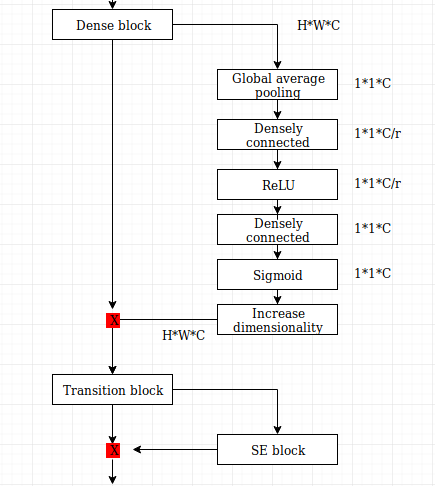
\includegraphics[width=0.8\textwidth]{background/sedense.png}
    \caption{}
    \label{figure:background:sedense}
\end{figure}

To get a better growth rate and number of dense layers we trained our model with 3 number of dense layers configurations [6,12], [6,12,16] and [6,12,24,16] where each number of the list is the amount of dense layers that will fit in each dense block separated with transition blocks. For each number of dense layers configuration we trained with different growth rate, this way we prevented memory errors and getting the neural network to grow too large or too small. For [6,12] we trained with a growth rate of 64 and 128 and for [6,12,16] and [6,12,24,16] we trained with 32 and 64 growth rate. \\

We split the dataset in training and test with the test set taking \%33 of the images and the training set the remaining images. For data augmentation we used flipping, a 10 and 30 degree rotation and a rescaling of \%20 max. We found that a 10 degree rotation gave better results because a rotation of 30 degrees showed to be too high for the nature of the dataset. \\

The best configurations we got for the dataset without data augmentation is a growth rate of 128 and a number of dense layers of [6,12]. With data augmentation, the best configuration we got is 64 growth rate and [6,12] number of dense layers.

\subsection{RWTH}

\subsubsection{Data analysis}

There is a clear class imbalance due to the origin of the images, ranging from classes with 1 sample to classes with 529 samples. We decided to remove all the classes that had less than 20 samples to have a solid amount of images per class for our networks to learn, after removing the images we relabeled them to make their numerical class label fit the amount of classes in the filtered dataset. There is some movement blur on some images. Some images contain both hands of the interpreter and some images don't have the hand perfectly centered.

\subsubsection{Prototypical Network}

We use the same four-block embedding architecture as in our LSA16 experiments by adding an eight-block architecture with the same layer composition with the idea of analyzing the variation of performance with the growth of the network. \\

The difference in the results obtained in 1-shot and 5-shot scenarios for this dataset was very large. We found that 5-shot scenarios gave better results. Using this discovery we only used 5-shot learning in the remaining experiments. \\

We used the same model, train-test split and data augmentation that we used in the previous dataset. \\

We got the best configurations in the 5-shot scenarios with equals training-shot and test-shot by using more than or equal to 5 classes (way) per training episode. The best configurations of the embedding architecture is a 64-filter.

\subsubsection{Dense Network}

This is the first model with which we searched for good hyperparameters in densenet. We searched with a reduction of 0 and 0.5. We found that a 0.5 reduction gave better results. Using this discovery we only used a 0.5 reduction in the search for better hyperparameters in the rest of the datasets. \\

We used the same model, train-test split and data augmentation that we used in the previous dataset. \\

The best configurations we got for the dataset without data augmentation is a growth rate of 32 and a number of dense layers of [6,12,16]. With data augmentation, the best configuration we got is 64 growth rate and [6,12] number of dense layers. 

\subsection{CIARP}

The hands are centered and were extracted from the background, the images are presented in a black background.
The small images and the low amount of classes give this dataset lower complexity compared to LSA16 and RWTH.

\subsubsection{Data analysis}

\subsubsection{Prototypical Network}

We use the same four-block embedding architecture as in our LSA16 experiments. \\

We used the same model, train-test split and data augmentation that we used in the previous dataset. We trained prototypical networks only in the 5-shot scenarios. \\

We got the best configurations with equals training-shot and test-shot by using more than or equal to 5 classes (way) per training episode. Better results were obtained when the number of classes approaches the total amount of classes. In addition, the best configurations of the embedding architecture is a 64-filter.

\subsubsection{Dense Network}

Because of the little and the small amount of classes, we decided to search for the best hyperparameters in the combination of 64 or 128 growthrate with [6,12] number of dense layers. \\

We used the same model, train-test split and data augmentation that we used in the previous dataset. \\

The best configurations we got for the dataset with and without data augmentation is a growth rate of 32 and a number of dense layers of [6,12].

\subsection{Results}

\begin{table}[h!]
\centering
\begin{tabular}{ p{18em} p{7em} p{8em} p{8em}}
\toprule
\emph{Method} & \emph{LSA16} &  \emph{RWTH}  &  \emph{CIARP} \\ \midrule
CIARP pAPER (https://link.springer.com/chapter/10.1007/978-3-319-75193-1\_53)* \cite{CIARP_resultados} & - & - &  \\
DeepHand* \cite{koller2016deep} & - & 85.50 \\
VGG16* \cite{Quiroga_blablabla} & 95.92 & 82.88 \\
DenseNet \cite{} & 93.79 & \textbf{90.51} & NN.NN \\
Prototypical Networks \cite{} & 97.86 & 75.23 & 99.96 \\
DenseNet ++ \cite{} & 96.45 & 86.23 & NN.NN \\
Prototypical Networks ++\cite{} & \textbf{97.99} & 75.94 & 99.99  \\
DenseNet + Unlabeled \cite{} & NN.NN & NN.NN \\
Prototypical Networks + Unlabeled \cite{} & NN.NN & NN.NN \\
\bottomrule
\end{tabular}
\caption{Accuracy of various convolutional neural network models on three datasets: LSA16 \cite{ronchetti2016a}, handshapes from RWTH-PHOENIX-Weather \cite{koller2016deep} and CIARP. Results from methods annotated with * were taken from other papers. Models with "++" used data augmentation as described in section XXXX. \label{tab:results}}
\end{table}

\section{Conclusion}

\section{Trabajos futuros}
AUTOAUGMENT [https://arxiv.org/abs/1805.09501]
hand tracking
https://www.analyticsvidhya.com/blog/2017/09/pseudo-labelling-semi-supervised-learning-technique/
https://arxiv.org/pdf/1812.08781.pdf
https://arxiv.org/abs/1906.00562

\begin{thebibliography}{4}
    \bibitem{matchingnet} \href{https://arxiv.org/abs/1606.04080}{Matching Networks for One Shot Learning}. Oriol Vinyals, Charles Blundell, Timothy Lillicrap, Koray Kavukcuoglu, Daan Wierstra.
    \bibitem{protonet} \href{https://arxiv.org/abs/1703.05175}{Prototypical Networks for Few-shot Learning}. Jake Snell, Kevin Swersky, Richard S. Zemel.
    \bibitem{omniglot} \href{https://github.com/brendenlake/omniglot}{Omniglot dataset}.
    \bibitem{densenet} \href{https://arxiv.org/pdf/1608.06993.pdf}{Densely Connected Convolutional Networks}. Gao Huang et al.
    \bibitem{resnet} \href{https://arxiv.org/pdf/1512.03385.pdf}{Deep Residual Learning for Image Recognition}. Kaiming He et al.
    \bibitem{densenet_cifar} \href{https://arxiv.org/pdf/1802.03268.pdf}{Efficient Neural Architecture Search via Parameter Sharing}. Hieu Pham et al.
    \bibitem{senet} \href{https://arxiv.org/pdf/1709.01507.pdf}{Squeeze-and-Excitation Networks}
    \bibitem{data_augmentation} \href{https://books.google.com.ar/books?id=rERADwAAQBAJ&pg=PA64&lpg=PA64&dq=Variance+is+the+algorithm\%E2\%80\%99s+tendency+to+learn+random+things+irrespective+of+the+real+signal+by+fitting+highly+flexible+models+that+follow+the+error&source=bl&ots=raekkRHUoA&sig=ACfU3U0m3wuVS6hW9WDDsq4SGP8rSDK6Fg&hl=es-419&sa=X&ved=2ahUKEwjw8Z73q4rjAhVvD7kGHa4jDnwQ6AEwBXoECAkQAQ#v=onepage&q&f=false}{Machine Learning with R}. Abhijit Ghatak.
    \bibitem{wide_resnet}
    \href{https://arxiv.org/pdf/1605.07146.pdf}{Wide Residual Networks}. Sergey Zagoruyko, Nikos Komodakis.
\end{thebibliography}

\end{document}
